\section{Anchor distances}
\subsection{andi}

\newcommand{\anchor}[6]{
    \fill[#5, opacity=0.2] 
      (#1,3) -- (#2,3) -- (#4,0) -- (#3,0) -- cycle;
    \node[above] at ({(#1+#2)/2}, 3) {#6};
    \node[below] at ({(#3+#4)/2}, 0) {#6};
}
\newcommand{\spanchor}[5]{
    \node[above] at ({(#1+#2)/2}, 3) {#5};
    \node[below] at ({(#3+#4)/2}, 0) {#5};
}
\newcommand{\spoben}[3]{
    \node[above] at ({(#1+#2)/2}, 3) {#3};
}
\newcommand{\spunten}[3]{
     \node[below] at ({(#1+#2)/2}, 0) {#3};
}

\begin{figure}[H]
    \centering
    \resizebox{17cm}{!}{
    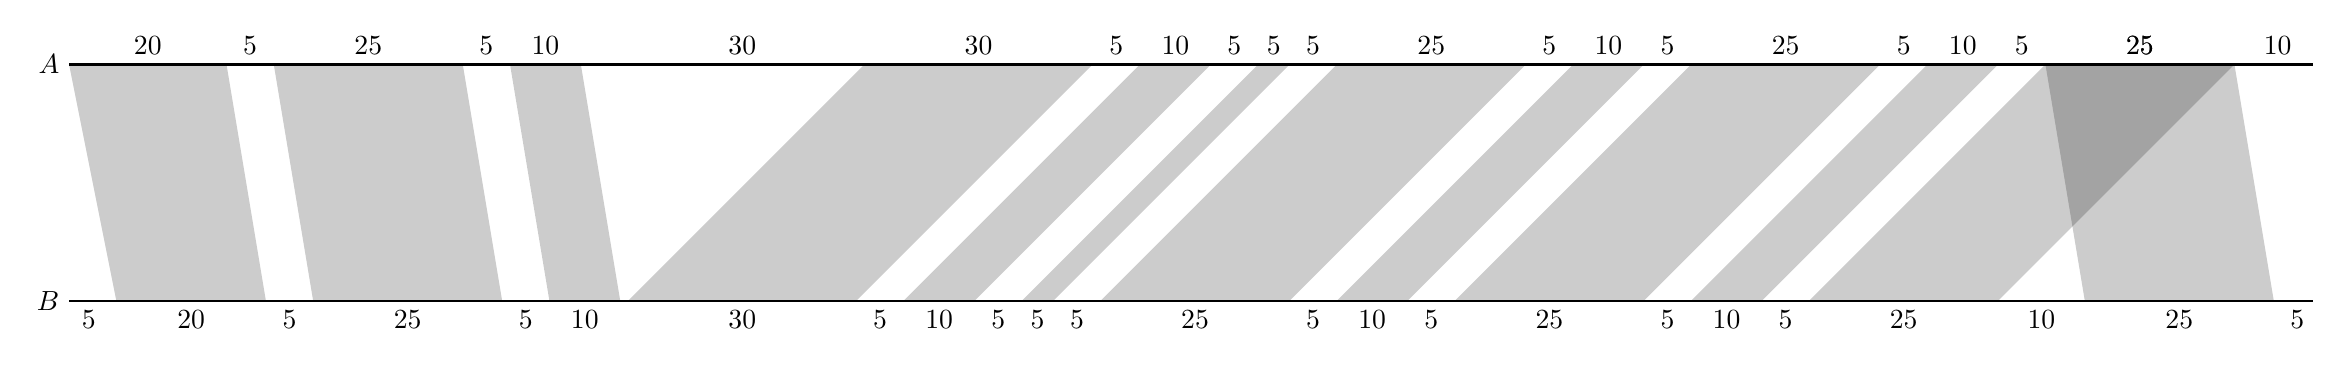
\begin{tikzpicture}

  % (q_start, q_end, s_start, s_end)
  \spunten{0}{0.5}{5}
  \anchor{0}{2.0}{0.6}{2.5}{black}{20}
  \spanchor{2.1}{2.5}{2.6}{3.0}{5}
  \anchor{2.6}{5.0}{3.1}{5.5}{black}{25}
  \spanchor{5.1}{5.5}{5.6}{6.0}{5}
  \anchor{5.6}{6.5}{6.1}{7.0}{black}{10}
  \spoben{7.1}{10.0}{30} 
  \anchor{10.1}{13.0}{7.1}{10.0}{black}{30}
  \spanchor{13.1}{13.5}{10.1}{10.5}{5}
  \anchor{13.6}{14.5}{10.6}{11.5}{black}{10}
  \spanchor{14.6}{15}{11.6}{12}{5}
  \anchor{15.1}{15.5}{12.1}{12.5}{black}{5}
  \spanchor{15.6}{16}{12.6}{13}{5}
  \anchor{16.1}{18.5}{13.1}{15.5}{black}{25}
  \spanchor{18.6}{19}{15.6}{16}{5}
  \anchor{19.1}{20}{16.1}{17}{black}{10}
  \spanchor{20.1}{20.5}{17.1}{17.5}{5}
  \anchor{20.6}{23}{17.6}{20}{black}{25}
  \spanchor{23.1}{23.5}{20.1}{20.5}{5}
  \anchor{23.6}{24.5}{20.6}{21.5}{black}{10}
  \spanchor{24.6}{25}{21.6}{22}{5}
  \anchor{25.1}{27.5}{22.1}{24.5}{black}{25}
  \spunten{24.6}{25.5}{10}
  \anchor{25.1}{27.5}{25.6}{28}{black}{25}
  \spoben{27.6}{28.5}{10}
  \spunten{28.1}{28.5}{5}



  \draw[thick] (0,3) -- (28.5,3);
  \node[left] at (0,3) {$A$};

  \draw[thick] (0,0) -- (28.5,0);
  \node[left] at (0,0) {$B$};

\end{tikzpicture}
}
    \caption{Anchor distance example from exercise 11.}
    \label{fig:my_label}
\end{figure}

\noindent We calculate $n$ and $s$ for every group of anchors that shares the same of spacing and from that we calculate the JC-Correction. 
\begin{figure}[H]
    \centering
    \resizebox{17cm}{!}{
    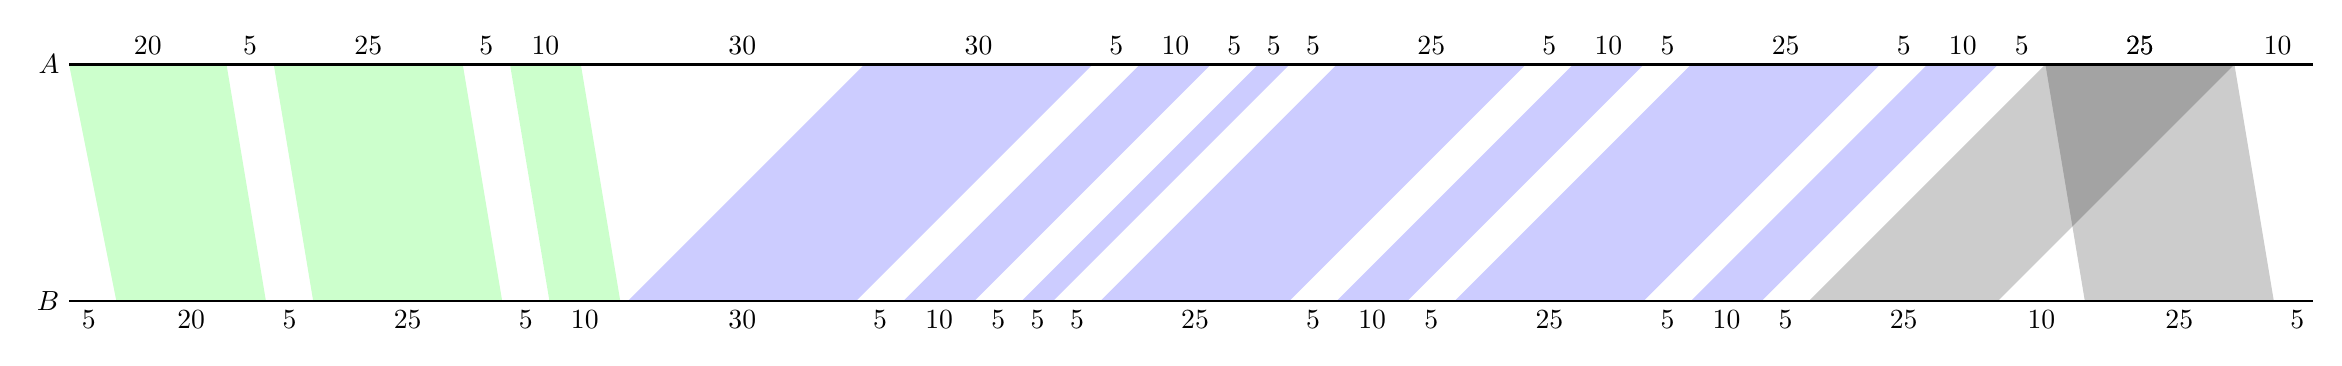
\begin{tikzpicture}


  % (q_start, q_end, s_start, s_end)
  \spunten{0}{0.5}{5}
  \anchor{0}{2.0}{0.6}{2.5}{green}{20}
  \spanchor{2.1}{2.5}{2.6}{3}{5}
  \anchor{2.6}{5.0}{3.1}{5.5}{green}{25}
  \spanchor{5.1}{5.5}{5.6}{6.0}{5}
  \anchor{5.6}{6.5}{6.1}{7.0}{green}{10}
  \spoben{7.1}{10.0}{30} 
  \anchor{10.1}{13.0}{7.1}{10.0}{blue}{30}
  \spanchor{13.1}{13.5}{10.1}{10.5}{5}
  \anchor{13.6}{14.5}{10.6}{11.5}{blue}{10}
  \spanchor{14.6}{15}{11.6}{12}{5}
  \anchor{15.1}{15.5}{12.1}{12.5}{blue}{5}
  \spanchor{15.6}{16}{12.6}{13}{5}
  \anchor{16.1}{18.5}{13.1}{15.5}{blue}{25}
  \spanchor{18.6}{19}{15.6}{16}{5}
  \anchor{19.1}{20}{16.1}{17}{blue}{10}
  \spanchor{20.1}{20.5}{17.1}{17.5}{5}
  \anchor{20.6}{23}{17.6}{20}{blue}{25}
  \spanchor{23.1}{23.5}{20.1}{20.5}{5}
  \anchor{23.6}{24.5}{20.6}{21.5}{blue}{10}
  \spanchor{24.6}{25}{21.6}{22}{5}
  \anchor{25.1}{27.5}{22.1}{24.5}{black}{25}
  \spunten{24.6}{25.5}{10}
  \anchor{25.1}{27.5}{25.6}{28}{black}{25}
  \spoben{27.6}{28.5}{10}
  \spunten{28.1}{28.5}{5}



  \draw[thick] (0,3) -- (28.5,3);
  \node[left] at (0,3) {$A$};

  \draw[thick] (0,0) -- (28.5,0);
  \node[left] at (0,0) {$B$};

\end{tikzpicture}
}
    \caption{Colourisation of anchor distance example from exercise 11 in regards to A as the Query: $n_1 = 50$, $s_1 = 5$ (green) and $n_2 = 130$, $s_2 = 50$ (blue). $K(A,B)=JC\big( \frac{5+50}{130+50} \big)=JC\big( \frac{55}{180} \big) \approx 0.392$.}
    \label{fig:my_label}
\end{figure}

\begin{figure}[H]
    \centering
    \resizebox{17cm}{!}{
    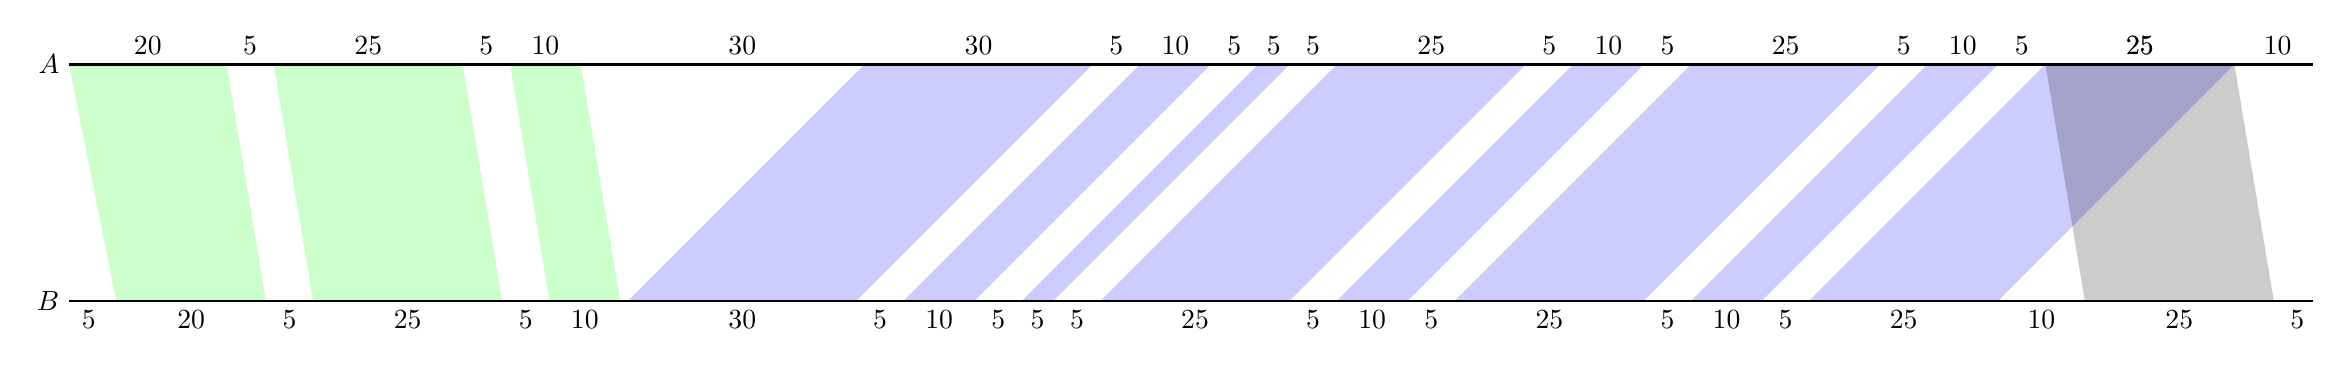
\begin{tikzpicture}


  % (q_start, q_end, s_start, s_end)
  \spunten{0}{0.5}{5}
  \anchor{0}{2.0}{0.6}{2.5}{green}{20}
  \spanchor{2.1}{2.5}{2.6}{3}{5}
  \anchor{2.6}{5.0}{3.1}{5.5}{green}{25}
  \spanchor{5.1}{5.5}{5.6}{6.0}{5}
  \anchor{5.6}{6.5}{6.1}{7.0}{green}{10}
  \spoben{7.1}{10.0}{30} 
  \anchor{10.1}{13.0}{7.1}{10.0}{blue}{30}
  \spanchor{13.1}{13.5}{10.1}{10.5}{5}
  \anchor{13.6}{14.5}{10.6}{11.5}{blue}{10}
  \spanchor{14.6}{15}{11.6}{12}{5}
  \anchor{15.1}{15.5}{12.1}{12.5}{blue}{5}
  \spanchor{15.6}{16}{12.6}{13}{5}
  \anchor{16.1}{18.5}{13.1}{15.5}{blue}{25}
  \spanchor{18.6}{19}{15.6}{16}{5}
  \anchor{19.1}{20}{16.1}{17}{blue}{10}
  \spanchor{20.1}{20.5}{17.1}{17.5}{5}
  \anchor{20.6}{23}{17.6}{20}{blue}{25}
  \spanchor{23.1}{23.5}{20.1}{20.5}{5}
  \anchor{23.6}{24.5}{20.6}{21.5}{blue}{10}
  \spanchor{24.6}{25}{21.6}{22}{5}
  \anchor{25.1}{27.5}{22.1}{24.5}{blue}{25}
  \spunten{24.6}{25.5}{10}
  \anchor{25.1}{27.5}{25.6}{28}{black}{25}
  \spoben{27.6}{28.5}{10}
  \spunten{28.1}{28.5}{5}



  \draw[thick] (0,3) -- (28.5,3);
  \node[left] at (0,3) {$A$};

  \draw[thick] (0,0) -- (28.5,0); 
  \node[left] at (0,0) {$B$};

\end{tikzpicture}
}
    \caption{Colourisation of anchor distance example from exercise 11 in regards to B as the Query: $n_1 = 50$, $s_1 = 5$ (green) and $n_2 = 175$, $s_2 = 70$ (blue). $K(B,A)=JC\big( \frac{5+70}{175+50} \big)=JC\big( \frac{75}{225} \big) \approx 0.441$.}
    \label{fig:my_label}
\end{figure}

\noindent from that, we can calculate the anchor distance $Dist = \frac{K(A,B) + K(B,A)}{2} \approx 0.4165$.

%\begin{table}[H]
%    \centering
%    \begin{tabular}{c|ccc ccc ccc c}
%        \textbf{Iteration} & $q_c$ & $q_p$ & $s_c$ & $s_p$  &$l_c$ & $l_p$ & $s$ & $n$ & $a$ & $m$\\ \hline
%         Init& 1 & 1 & 1 & 1 & 0 & 0 & 0 & 0 & f & null \\ 
%         I & 22 & 1 & 6 & 6 & 21 & 21 & 0 & 0 & f & A[1-20] \\
%         II & qc & qp & sc & sp & lc & lp & s & n & a & m \\
%         I & qc & qp & sc & sp & lc & lp & s & n & a & m \\
%    \end{tabular}
%    \caption{Query: A, Subject: B}
%    \label{tab:my_label}
%\end{table}

\subsubsection{Link to andi visualisation}
\url{https://evolbioinf.github.io/andi/}